%%%%%%%%%%%%%%%%%%%%%%%%%%%%%%%%%%%%%%%%%%%%%%%%%%%%%%%%%%%%%%%%%%%%%%
% How to use writeLaTeX: 
%
% You edit the source code here on the left, and the preview on the
% right shows you the result within a few seconds.
%
% Bookmark this page and share the URL with your co-authors. They can
% edit at the same time!
%
% You can upload figures, bibliographies, custom classes and
% styles using the files menu.
%
%%%%%%%%%%%%%%%%%%%%%%%%%%%%%%%%%%%%%%%%%%%%%%%%%%%%%%%%%%%%%%%%%%%%%%

\documentclass[12pt]{article}

\usepackage{sbc-template}

\usepackage{graphicx,url}

\usepackage[brazil]{babel}   
\usepackage[utf8]{inputenc}
\usepackage{graphicx}
\usepackage[portuguese, linesnumbered]{algorithm2e}
\usepackage{amsthm}
\usepackage{tabularx}
\usepackage{booktabs}

     
\sloppy

\title{HAIL: um modelo de revisão de percepções\\de agentes inteligentes baseado em alucinação e ilusão}

\author{Gustavo E. Kundlatsch\inst{1}, Thiago Ângelo Gelaim\inst{1}, Elder Santos\inst{1} }


\address{Departamento de Informática e Estatıstica\\
Universidade Federal de Santa Catarina (UFSC)\\
Florianópolis -- SC -- Brazil}

\theoremstyle{definition}
\newtheorem{definition}{Definição}
\newtheorem{example}{Exemplo}[section]

\newcolumntype{Y}{>{\centering\arraybackslash}X}
\newcolumntype{P}[1]{>{\centering\arraybackslash}p{#1}}
\newcommand{\centered}[1]{\begin{tabular}{l} #1 \end{tabular}}

\begin{document} 

\maketitle

\begin{abstract}
  Perceptions are the main way to an entity to receive information from the environment. Each person has a different manner of percept and interpretate the world. However, it is known that in the human perception there are anomalies, incorrect perceptions that decieve the mind. So, how can we know if our perceptions are real or just tricks from our mind? And the follow up question is: what about computers? Inteligent agents are computational entities capable of making decisions based on the environment, and use sensors to perceive the world. But sensors can fail. In the current work, we present a generic model of perception revision, capable of treating anomalies received by the agent and creating new plans from them to adapt to the environment. This model was implemented and submited to experiments to test it's behavior. The simulations demonstrate that the model is capable of detect and classify anomalies and that in environments with a high amount of anomalies the model can have more inpact creating new plans through the automatic planning process and increasing the amount of valid perceptions received by the agent's cognition.
\end{abstract}
     
\begin{resumo} 
  Percepções são a principal maneira de uma entidade receber informações do ambiente. Cada pessoa possui uma maneira diferente de perceber e interpretar o mundo. Entretanto, sabe-se que na percepção humana existem anomalias, que são percepções incorretas que enganam a mente. Dito isso, como podemos saber se nossas percepções são reais ou se são apenas fruto de nossa imaginação? E a questão derivada disso é: e computadores? Agentes inteligentes são entidades computacionais autônomas capazes de tomarem decisões baseadas no ambiente no qual estão inseridos, e utilizam sensores para reconhecerem o mundo a sua volta. Mas esses sensores podem falhar. Neste trabalho, apresentamos um modelo genérico de revisão de percepções, capaz de tratar anomalias recebidas pelo agente e criar novos planos a partir delas para se adaptar ao ambiente. Esse modelo foi implementado e submetido a experimentos para testar seu funcionamento. As simulações realizadas demonstraram que o modelo é capaz de detectar e classificar as anomalias e que em ambientes com grande quantidade de anomalias o modelo consegue ter maior impacto criando novos planos através do planejamento automatizado e aumentando a quantidade de percepções válidas recebidas pelo raciocínio do agente.
\end{resumo}

\section{Introdução}

Dentro da Inteligência Artificial (IA), agentes inteligentes são entidades capazes de raciocinar a respeito do ambiente em que estão inseridos e tomar decisões baseadas na situação em que se encontram \cite{russell2016artificial}. Dessa maneira, podemos descrever um agente pelo seus processos de percepção, raciocínio e atuação. O agente ocupa um ambiente, do qual recebe informações e no qual atua. O ambiente é o mundo em que o agente está inserido, podendo ser uma construção virtual como uma simulação ou uma parte do mundo real, no caso de um agente físico. Existem diversos tipos de ambientes que podem ser classificados de acordo com o seu fechamento (que determina se agentes de fora do ambiente podem afetar o sistema), dinamismo (a maneira como o ambiente evolui), determinismo (a consistência dos efeitos no ambiente) e cardinalidade (o número de objetos a serem afetados e percebidos) \cite{moya2007towards}.

Uma das maneiras de um agente atualizar seu conhecimento a respeito do ambiente é a percepção, o processo de utilizar sensores para detectar o ambiente e transformar os dados coletados em informações úteis \cite{weyns2004towards}.  O raciocínio, por sua vez, é o processamento das percepções baseado nos objetivos do agente, que resulta em um conjunto ações a serem tomadas através dos atuadores. O processo do raciocínio é comandado pela arquitetura cognitiva do agente, um modelo computacional inspirado na estrutura da mente humana \cite{DYACHENKO2018130}. As arquiteturas cognitivas podem ser divididas em três categorias: simbólicas, emergentes e híbridas \cite{yeCognitivearchitectures}. Arquiteturas simbólicas descrevem o ambiente através de símbolos armazenados em memória em uma base de conhecimentos, e utilizam lógica simbólica para realizar o ciclo de percepção, raciocínio e ação. Arquiteturas emergentes se baseiam na estrutura biológica do cérebro e normalmente utilizam redes neurais em uma estrutura hierárquica para lidar com situações de incerteza. Por fim, arquiteturas híbridas combinam o comportamento emergente e o processamento simbólico para resolver problemas de diversos domínios. 

Todavia, sensores podem apresentar problemas para o processo de percepção por razões como campo de visão, distância do objeto observado, resolução dos sensores e leituras não confiáveis \cite{chrisman1991intelligent}. Tratar deste problema normalmente é responsabilidade da arquitetura cognitiva do agente, pois a arquitetura precisa ser capaz de fazer a ponte entre o ambiente e o conhecimento do agente \cite{langley2009cognitive}.

O objetivo deste trabalho é apresentar um modelo genérico (independente da arquitetura do agente) que pode ser acoplado entre o processo de percepção e raciocínio, capaz de detectar e tratar percepções inválidas para transformá-las em informações úteis através de um processo de criação de novos planos. Esse modelo pressupõe um ambiente aberto (onde agentes externos podem influenciar o ambiente), dinâmico (mudanças no ambiente são causadas por eventos aleatórios) e não determinístico (ações do agente causam resultados diferentes no ambiente, mesmo em situações aparentemente idênticas, pois os resultados variam dependendo da percepção do agente daquele evento).  
\section{Fundamentação teórica}

Alguns conceitos precisam ser bem definidos para que sejam utilizados mais tarde na formalização do modelo proposto. Esse capítulo apresenta essas definições iniciais.

\subsection{Agente inteligente}

Um agente inteligente é uma entidade autônoma, capaz de tomar as próprias decisões para atingir seus objetivos \cite{wooldridge1999intelligent}. Apesar da definição intuitiva ser simples, assim como no termo inteligência artificial não existe um consenso da comunidade sobre o que é um agente. Para este trabalho, compomos a seguinte formalização de agente inteligente:

\vspace{0.2cm}

\theoremstyle{definition}
\begin{definition}
    \label{def:agent}
    Um agente é uma tripla $Ag = \langle K, P, \gamma \rangle$, onde:
    \begin{itemize}
        \item $K$ é uma base de conhecimentos, tal que $K = K_i \cup K_p$, onde $K_i$ é o conjunto de conhecimentos inicias do agente e $K_p$ os conhecimentos adquiridos através das percepções. $K_i$ é iniciado com valores arbitrários de acordo com a necessidade do agente e $K_p$ é iniciado vazio. Uma base de conhecimentos é uma estrutura que representa fatos a respeito do mundo e apresenta formas de raciocinar a respeito desses fatos para deduzir novos conhecimentos \cite{hayes1983building};
        \item $P$ é o conjunto de planos do agente, sendo um plano definido como $plano = (\Psi, A, \Omega)$, onde $\Psi$ é o conjunto união formado pelas pré-condições das ações que compõem o plano, $A$ o conjunto de ações que compõe o plano e $\Omega$ o conjunto união formado pelas pós-condições das ações que compõem o plano. Por sua vez, uma ação é definida como $acao = (\psi, n, \omega)$, sendo $\psi$ um conjunto de pré-condições, $n$ um nome para a ação e $\omega$ um conjunto de pós-condições; e
        \item $\gamma$ é a função de percepção, definida como $ \gamma(p, K) \rightarrow P_i $, onde $p$ é o conjunto de percepções recebidas, $K$ a base de conhecimentos de $Ag$ e $P_i$ o retorno da função, que é um subconjunto próprio do conjunto $P$ de planos do agente.
    \end{itemize}{}
\end{definition}{}

A partir dessa definição, podemos construir o conceito de contexto, que será importante mais tarde para o modelo de revisão de percepções. O contexto de um agente é o conjunto de todos os símbolos compreendidos pelo agente, e cuja percepção de cada um desses símbolos resulta na execução de um conjunto de ações diretamente mapeadas.

\vspace{0.2cm}

\begin{definition}
    O contexto $c$ de um agente $Ag$ é o domínio de sua função $\gamma$.
    \label{definition::context}
\end{definition}{}

Para este trabalho, serão utilizados símbolos compostos para representar percepções e ações. Esses símbolos são formados da maneira \emph{predicado(caracteristica)}, onde o predicado é o elemento principal do símbolo e a característica uma propriedade secundária.

\subsection{Percepção}

Existem diversas definições para o termo ``percepção''. Podemos entender percepção como um conjunto de sensações que, através da maneira subjetiva que um dado agente o interpreta, representa determinadas entidades do ambiente \cite{gibson1950perception}. Ou seja, a percepção não é simplesmente a representação direta das entidades reais que existem no mundo, mas um processo complexo que varia para cada indivíduo.

Para o modelo que iremos propor, baseado na Definição \ref{def:agent}, o conceito de percepção pode ser simplesmente definido como as entradas da função de percepção $\gamma$ de um agente. Vale destacar a diferença entre percepção e contexto, pois o contexto é constituído pelas percepções que fazem parte do domínio da função $\gamma$, ou seja, uma percepção é toda informação produzida pelo ambiente que o agente recebe, e contexto é o subconjunto das percepções que o agente possui planos para tratar.

\subsubsection{Refinamento}

Como o volume de percepções de um agente pode ser muito grande, e as percepções tomam determinado tempo para serem processadas, o número de percepções que chegam ao ciclo de raciocínio do agente pode ser reduzido para diminuir seu custo computacional. Neste trabalho, esse processo será chamado de refinamento, definido da seguinte maneira:

\vspace{0.2cm}

\begin{definition}
    \label{def:refinamento}
    Refinamento de percepções é uma função $\theta$ tal que, dado o conjunto de entradas de percepções $p$, reduz tais percepções para um subconjunto próprio $\rho$.
\end{definition}

\subsubsection{Anomalias}

\label{anomalias}

Anomalias são as percepções consideradas inválidas, geradas por alguma falha no processo de percepção. Toda percepção para a qual o agente não possui uma resposta mapeada em sua função de percepção é considerada uma anomalia. O conjunto de anomalias de um agente é o conjunto de todas as percepções possíveis que não fazem parte de seu contexto. A seguinte definição será utilizada:

\vspace{0.2cm}

\begin{definition}
    Uma percepção $p$ de um agente $Ag$ com contexto $c$, é uma anomalia caso $p \notin c$ de $Ag$.
\end{definition}

Neste trabalho, as anomalias serão classificadas em dois grupos: alucinações e ilusões. Essa classificação foi inspirada no problema da percepção, um campo de estudo da filosofia \cite{perception-problem}.

Uma ilusão é uma percepção da forma \textit{predicado(caracteristica)} onde ou o predicado ou a característica não faz parte do contexto do agente, ou seja, é uma percepção parcialmente correta. Uma alucinação é uma uma percepção da forma \textit{predicado(caracteristica)} onde nem o predicado nem a característica faz parte do predicado, ou seja, a percepção pode ser semanticamente correta mas ela não deveria ter sido realizada pelo agente.

\subsection{Planejamento automatizado}

Planejamento automatizado é um dos problemas fundamentais da Inteligência Artificial. As motivações para usar o planejamento automatizado são a capacidade de utilizar recursos de planejamento acessíveis e eficientes e reproduzir uma parte do processo cognitivo humano com um componente totalmente integrado de comportamento deliberativo \cite{GHALLAB20041}.

Na Definição \ref{definition::autoplanning} é apresentada a noção abstrata de planejamento automático, descrita como um modelo conceitual simples que contém os elementos principais do problema, tendo sido originalmente apresentada por \cite{GHALLAB20041}.

\vspace{0.2cm}

\begin{definition}{}
\label{definition::autoplanning}
   % USAR MAIS TARDE PARA DEFINIR O BLOCO DE AUTOPLANEJAMENTO An automated planning block is a instance of the conceptual model of automated planning, described through the interaction between three components bellow \cite{GHALLAB20041}:
   Um modelo conceitual de planejamento automatizado é descrito como a interação entre os seguintes três componentes:
   
    \begin{itemize}
        \item Um sistema de transição de estados $\Sigma$, especificado por uma função de transição de estados $y$, de acordo com os eventos e ações que ele recebe. 
        \item Um $controlador$, que dado uma entrada de estados $s$ do sistema, fornece como saída uma ação de acordo com algum plano.
        \item Um $planejador$, que dado uma entrada de uma descrição de sistema $Z$, uma situação inicial e alguns objetivos, sintetiza um plano para o controlador a fim de alcançar o objetivo.
    \end{itemize}
    
    Um sistema de transição de estados $\Sigma$ é uma quádrupla $\Sigma = \langle S, A, E, \Gamma \rangle$, onde:
    
    \begin{itemize}
        \item $S = \{s_1, s_2, ..., s_{n}\}$ é um conjunto finito ou recursivamente enumerável de estados;
        \item $A = \{a_1, a_2, ..., a_{n}\}$ é um conjunto finito ou recursivamente enumerável de ações;
        \item $E = \{e_1, e_2, ..., e_{n}\}$ é um conjunto finito ou recursivamente enumerável de eventos; e 
        \item $\Gamma: S \times A \times E \rightarrow 2^S$ é uma função de transição de estados. 
    \end{itemize}
     
\end{definition}



\section{Trabalhos relacionados}

Existem diversas abordagens para otimizar as percepções recebidas por um agente, isto é, garantir que todas as informações coletadas pelos sensores sejam utilizadas da melhor maneira possível. Diversos artigos apresentam processos de detectar percepções inválidas e tratá-las, de maneira similar ao modelo que será proposto neste trabalho.

Por exemplo, no artigo \emph{Scalable perception for BDI-agents embodied in virtual environments} \cite{van2011scalable} é definido um \emph{framework} onde os objetos do ambiente são definidos por classes e características e se organizam de maneira hierárquica, e a partir dessa organização o \emph{framework} é capaz de decidir que tipo de percepções o agente deseja perceber de acordo com seus interesses, alterando dinamicamente ao longo do tempo.
 
Outro trabalho similar é o \emph{PMK -- a knowledge processing framework for autonomous robotics perception and manipulation} \cite{Diab_2019}, onde o objetivo dos autores foi criar um mapa de todas as percepções possíveis no ambiente, de maneira que todas as percepções recebidas pelo agente estivessem em seu contexto, evitando anomalias. Todavia, isso não é viável em cenários abertos ou de alta complexidade, pois o mapeamento necessário é extenso demais. O modelo de programação lógica K-CoPMan (\textit{Knowledge enabled Cognitive Perception for Manipulation} ou Percepção Cognitiva Ativada pelo Conheci-mento para Manipulação) apresenta uma maneira do agente criar sua própria base de conhecimentos a partir da percepção passiva, eliminando as anomalias conforme elas são adicionadas ao contexto \cite{pangercic2010}.

Esses exemplos são de artigos que buscam otimizar as percepções recebidas pelo agente de maneira simbólica, mas esse problema pode ser abordado de maneira conexionista também. No artigo \emph{Understanding human intention by connecting perception and action learning in artificial agents} \cite{kim2017understanding} os autores propõem um modelo, chamado OA-SMTRNN (\textit{Object Augmented Supervised Multiple Timescale
Recurrent Neural Network}), para entender a intenção do usuário e responder ativamente da maneira mais adequada, através do uso de redes neurais. Para implementar o reconhecimento de intenção, são focados dois processos cognitivos, a percepção da disponibilidade de objetos e a previsão da ação humana. Com o uso de redes neurais, a ideia é extrair semântica de percepções que seriam inicialmente inválidas para o agente.

O objetivo do modelo proposto neste trabalho é detectar anomalias de maneira simbólica, classificando as percepções recebidas com o uso do contexto do agente como referencial, para então utilizar um processo de planejamento automatizado para gerar novos planos para o agente a partir das percepções inválidas.
\section{Modelo proposto}

O modelo proposto foi inspirado pelos conceitos de ilusão e alucinação apresentados na Seção \ref{anomalias}, que o nomeiam -- o nome HAIL vem da junção das palavras \textit{hallucination} e \textit{illusion}, alucinação e ilusão em inglês, respectivamente. Seu objetivo é identificar anomalias nas percepções recebidas por um agente qualquer e torná-las informação úteis na forma de novos planos.

O modelo HAIL foi desenvolvido para que seja possível adicioná-lo a qualquer agente, independente de arquitetura cognitiva, como um componente que conecta as percepções vindas do ambiente ao agente. O HAIL pode ser separado em dois módulos, como mostra a Figura \ref{fig:method}. De maneira geral, o funcionamento e a comunicação desses módulos se dá da seguinte maneira:

\begin{enumerate}
    \item As percepções recebidas pelo modelo são refinadas pelo módulo de refinamento;
    \item As percepções refinadas passam pelo módulo de alucinação e ilusão onde são categorizadas entre:  percepções válidas, alucinações, ilusões classe 1 e ilusões classe 2. 
    \item As percepções válidas são encaminhadas para o raciocínio do agente, enquanto as anomalias continuam no módulo de alucinação e ilusão armazenadas em estruturas chamadas de bloco avaliador;
    \item Quando os requisitos estabelecidos pelo bloco avaliador são cumpridos, as anomalias são selecionadas para passarem pelo processo de planejamento automatizado, alimentando o agente com novos planos.
\end{enumerate}
    
\begin{figure}[h!]
    \centering
    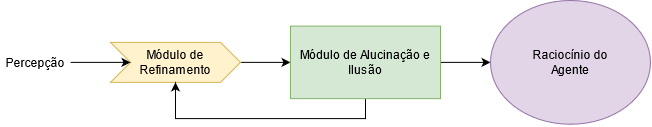
\includegraphics[width=1\textwidth]{images/modelo_geral.png}
    \caption{Visão geral do modelo HAIL.}
    \label{fig:method}
\end{figure}

\subsection{Módulo de refinamento}

\label{refinamento}

O módulo de refinamento funciona como uma primeiro filtro para que percepções indesejadas pelo agente não cheguem até seu ciclo de raciocínio. O processo de refinamento é descrito pela Definição \ref{def:refinamento}.

O processo de refinamento não é obrigatório. Caso não seja de interesse de uma determina implementação do HAIL refinar suas percepções, basta que a função do módulo de refinamento seja a função identidade $f(x) = x$, possuindo assim $\rho = p$.

\subsection{Módulo de alucinação e ilusão}

\begin{figure}[h]
    \centering
    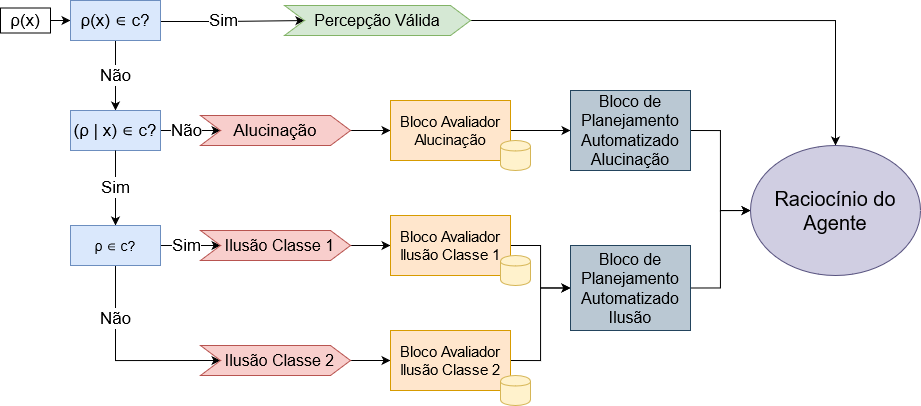
\includegraphics[width=1\textwidth]{images/diagrama-modelo.png}
    \caption{Módulo de alucinação e ilusão.}
    \label{fig:model}
\end{figure}
 
 A Figura \ref{fig:model} apresenta um diagrama do funcionamento do módulo de alucinação e ilusão. Sua função é receber todas as percepções que passaram pelo processo de refinamento, e detectar quais delas são anomalias. Para isso, esse módulo utiliza uma cadeia de decisores descrita pelo Algoritmo \ref{algorithm:decisor}. Depois de serem classificadas pelos decisores, as anomalias são guardadas em seus respectivos blocos avaliadores.

\begin{algorithm}[H]
\Entrada{contexto \textit{c} do agente, percepção $\rho(x)$}
\Inicio{
 \label{algorithm:decisor}
  \uSe{$\rho(x)$ está em \textit{c}}{
  $\rho(x)$ é uma percepção válida\;
  }\uSenaoSe{nem $\rho$ nem $x$ estão em c}{
  $\rho(x)$ é uma alucinação\;
  }\uSenaoSe{$\rho$ está em \texttt{c}}{
  $\rho(x)$ é uma ilusão classe 1\;
  }\Senao{$\rho(x)$ é uma ilusão classe 2}
}
 \caption{Funcionamento dos decisores do módulo de alucinação e ilusão.}
\end{algorithm}

\subsubsection{Bloco avaliador}

O objetivo do bloco avaliador é decidir quando alucinações e ilusões que foram recebidas devem ser processadas, evitando que o planejamento automatizado que será realizado em seguida tenha impacto no tempo de execução de um ciclo de raciocínio do agente. Para isso, utilizamos uma lista ordenada por peso como escalonador. O principio do funcionamento da lista ordenada por peso é o mesmo de uma fila, \textit{first in first out} (FIFO), mas atribui um peso a cada entrada que aumenta quando novos elementos iguais são inseridos. Quando um elemento é inserido pela primeira vez na fila, ele recebe o peso 1, e quando uma cópia do mesmo elemento é inserida o elemento tem seu peso aumentado em 1. Quando uma operação de remoção é executada, o elemento de maior peso é removido. Se dois ou mais elementos tiverem o maior peso, aquele que foi inserido primeiro é removido.

O bloco avaliador seleciona quando uma percepção deve ser tratada através de uma função matemática, levando em conta o tempo médio de processamento de uma percepção válida e de uma anomalia. Além desse funcionamento básico, o bloco avaliador ainda contém um mecanismo para remover anomalias classificadas com irrelevantes para o sistema, através de uma função de limpeza. Caso essa função retorne verdadeiro, todos os elementos de peso 1 da sua respectiva lista são removidos. Essas duas funções são descritas com mais detalhes na Seção \ref{section:formalizacao}.

\subsubsection{Bloco de planejamento automatizado}

O bloco de planejamento automatizado é potencialmente a parte mais custosa computacionalmente, o que pode ser um gargalo do sistema, principalmente caso o agente funcione em tempo real e receba um volume muito elevado de percepções por segundo. Um planejamento automatizado implementado de maneira puramente simbólica tende a ser complexo computacionalmente, uma vez que pode considerar milhares de alternativas para o estado de mundo atual, tentando chegar mais perto de seu objetivo. Um processo de planejamento automatizado conexionista é uma alternativa, uma vez que estamos tratando de uma análise incompleta do mundo. Caso seja possível, teorias com maior custo computacional (como criatividade computacional \cite{colton2012computational}) podem ser aplicadas aqui para um resultado ainda mais preciso.

Uma percepção chega ao bloco de planejamento automatizado uma vez que ela seja a primeira na fila ponderada e a função de processamento retorne verdadeiro em sua verificação. De um ciclo para outro, as percepções permanecem na fila, a não ser que sejam descartadas pelo mecanismo de limpeza. Nosso modelo não explicita qual é a ordem que os blocos avaliadores devem processar suas filas para mandar anomalias para o planejamento automatizado (isto é, se deve primeiro ser priorizada as anomalias do bloco avaliador de alucinações, ilusões classe 1 ou ilusões classe 2), ficando a cargo da implementação em questão tomar essa decisão.

\subsection{Formalização}

\label{section:formalizacao}

O bloco básico do modelo de revisão de percepções proposto, chamado de HAIL, é composto por um módulo para alucinação e ilusão $M_{ai}$ e uma função de refinamento $\theta$, conforme descrito na Definição \ref{def:modeloHAIL}. O módulo de ilusão e alucinação é uma quádrupla, apresentada na definição \ref{def:illuHallu}. A função de refinamento é uma função abstrata, cuja entrada é obtida através dos sensores do agentes e a saída é a entrada do módulo de alucinação e ilusão, conforme já foi descrito anteriormente na Seção \ref{refinamento}.
 
 \vspace{0.2cm}
 
 \begin{definition}{}
    O modelo de revisão de percepções HAIL é uma dupla $HAIL = \langle M_{ai}, \theta \rangle$, onde:
    
    \begin{itemize}
        \item $M_{ai}$ é o módulo de ilusão e alucinação; e
        \item $\theta$ é a função de refinamento $\theta(p) = \rho$, onde $p$ é um conjunto de percepções e $\rho$ é um subconjunto próprio de $p$.
    \end{itemize}{}
    \label{def:modeloHAIL}
\end{definition}

Após ter passado pela função $\theta$, as percepções $\rho$ irão passar pelo Algoritmo \ref{algorithm:decisor}, e serão encaminhadas de acordo com sua classificação. O bloco de ilusão e alucinação é descrito por uma quádrupla, com conjuntos de decisores, blocos e uma função de transição.

\vspace{0.2cm}

\begin{definition}
\label{def:illuHallu}
    O bloco de ilusão e alucinação é uma quádrupla $M_{ai} = \langle D, Ab, Ap, \Delta \rangle$, onde:
    
    \begin{itemize}
        \item $D$ é o conjunto de decisores $D = \{d_{a}, d_{h}, d_{i}\}$, onde:
             \begin{itemize}
                \item $d_{a}$ é o decisor de anomalias, definido pela função:
                \[ d_{a} = \left\{ \begin{array}{ll}
                0 & \mbox{se $\rho(x)$ está em $c$\footnotemark};\\
                1 & \mbox{se $\rho(x)$ não está em $c$}.\end{array} \right. \]
             
                \item $d_{h}$ é o decisor de alucinação, definido pela função:
                \[ d_{h} = \left\{ \begin{array}{ll}
                0 & \mbox{se nem $\rho$ nem $(x)$ está em $c$};\\
                1 & \mbox{se $\rho$ ou $(x)$ está em $c$}.\end{array} \right. \]
                
                \item $d_{i}$ é o decisor de ilusão, definido pela função:
                \[ d_{i} = \left\{ \begin{array}{ll}
                0 & \mbox{se $\rho$ está em $c$};\\
                1 & \mbox{se $(x)$ está em $c$}.\end{array} \right. \]
            \end{itemize}
        
        \footnotetext{ $c$ é o contexto do agente, de acordo com a definição \ref{definition::context}.}
        
        \item $Ab$ é o conjunto de blocos avaliadores $Ab = \{Ab_{h}, Ab_{i1}, Ab_{i2}\}$, onde $Ab_{h}$ é o bloco avaliador de alucinações, $Ab_{i1}$ é o bloco avaliador de ilusões classe 1 e $Ab_{i2}$ é o bloco avaliador de ilusões classe 2.
        
        \item $Ap$ é o conjunto de blocos de planejamento automatizado $Ap = \{Ap_{h}, Ap_{i}\}$, onde $Ap_{h}$ é o bloco de planejamento automatizado de alucinações e $Ap_{i}$ é o bloco de planejamento automatizado de ilusões.
        
        \item $\Delta$ é a função de transição definido pela tabela abaixo, onde $out$ é um estado final, que leva a percepção para fora do modelo de revisão de percepções, ou seja, pode tanto significar o encaminhamento de uma percepção válida para o raciocínio do agente quanto o fim da execução de um ciclo de revisão.
        
            \begin{table}[htb]
                \caption{Função de transição $\Delta$ do módulo de ilusão e alucinação.}
                \centering
                \begin{tabular}{c c c c} 
                    \toprule
                    \textbf{Estado} & \textbf{0} & \textbf{1} \\
                    \midrule
                    $d_{a}$     & $out$     & $d_{h}$       \\
                    $d_{h}$     & $Ab_{h}$  & $d_{i}$       \\
                    $d_{i}$     & $Ab_{i1}$ & $Ab_{i2}$     \\
                    $Ab_{h}$    & $out$     & $Ap_{h}$      \\
                    $Ab_{i1}$   & $out$     & $Ap_{i}$      \\
                    $Ab_{i2}$   & $out$     & $Ap_{i}$      \\
                    \bottomrule
                \end{tabular}
                \label{transition-table}
                
            \end{table}
    \end{itemize}{}
\end{definition}{}

O módulo de ilusão e alucinação é o artefato principal do modelo. Ele é subdividido em três partes principais: os decisores, os blocos avaliadores e os blocos de planejamento automatizado. Seu comportamento é descrito por uma função de transição que define o estado atual do módulo.

\vspace{0.2cm}

\begin{definition}
    Um bloco avaliador é uma tripla $Ab_{x} = \langle L, Pf, Cf) \rangle$, $x \in \{h, i1, i2\}$, onde:

    \begin{itemize}
        \item $L$ é uma lista ordenada pelo número de vezes que uma mesma anomalia é dada como entrada;
        \item $Pf$ é a função de processamento, definida abaixo:
            
             \[ Pf = \left\{ \begin{array}{ll}
                        1 & \mbox{se $T_{m}(A) \leq T_{m}(V) * (|A| - |A_{pr}|)$;}\\
                        0 & \mbox{caso contrário}.\end{array} \right. \]
        
            
            Onde:
            
            \begin{itemize}
                \item $T_{m}$ é a função que retorna a média do tempo gasto para processar as percepções de um conjunto;
                \item $A$ é o conjunto de anomalias, $A(x)$ é um elemento específico $x$ e $|A|$ o número de anomalias do conjunto;
                \item $A_{pr}$ é o conjunto de anomalias que já foram validadas para serem processadas pela função de processamento neste ciclo de raciocínio ($A_{pr}$ é instanciada vazia a cada ciclo de raciocínio), e $|A_{pr}|$ o número de anomalias desse conjunto.
                \item $V$ é o conjunto de percepções válidas.
            \end{itemize}{}
        
        \item $Cf$ é a função de limpeza definida abaixo com auxílio da função equação de limpeza $Cf$, sendo $\alpha$ um coeficiente de limpeza variável que precisa ser definido pela instância implementada do modelo (por padrão, toma-se $\alpha = 1$):
        
        \[ Cf = \left\{ \begin{array}{ll}
                        1 & \mbox{se  $Ce = Verdadeiro$;}\\
                        0 & \mbox{caso contrário}.\end{array} \right. \]
            
            \[ Ce = \sum_{i=1}^{|L|} W_{n}(L_{i}) > \alpha \sum_{j=1}^{|L|} W_{1}(L_{j}) \]
            
            Onde:
            
            \begin{itemize}
                \item $L$ é a lista ordenada do bloco, sendo $|L|$ seu número de anomalias e $L_{i}$ a anomalia $i$ da lista.
                \item $W$ é a função peso da anomalia $L_{i}$ definida como $W(L_{i}) = |L_{i}|$, sendo $|L_{i}|$ o peso da anomalia especificada (número de entradas recebidas dessa mesma anomalia na lista). A função $W$ é utilizada para especificar as seguintes funções:
                \\
                
                    (i) $ W_{1}(L_{i}) = \left\{ \begin{array}{ll}
                        1 & \mbox{se $W(L_{i}) = 1$;}\\
                        0 & \mbox{caso contrário}.\end{array} \right. $
                \\
                
                    (ii) $ W_{n}(L_{i}) = \left\{ \begin{array}{ll}
                        W(L{i}) & \mbox{se $W(L_{i}) > 1$;}\\
                        0 & \mbox{caso contrário}.\end{array} \right. $
            \end{itemize}{}
    \end{itemize}
\end{definition}{}

\vspace{0.2cm}

O bloco de planejamento automatizado recebe como entrada uma anomalia de um dos blocos avaliadores quando a função de processamento retorna verdadeiro, e pode ser definido da seguinte maneira:

\vspace{0.2cm}

\begin{definition}
    Um bloco de planejamento automatizado é uma instância do modelo conceitual de planejamento automatizado (Definição \ref{definition::autoplanning}).
\end{definition}


\section{Experimentos}

Para este trabalho foram realizados três experimentos com o objetivo de averiguar se o modelo HAIL é funcional ou não. Esses experimentos não possuem um domínio específico, ou seja, não há um ambiente real onde o agente está inserido, ele recebe percepções aleatórias geradas pelo simulador e os planos inicias do agente não são relevantes para os testes.

Os dois primeiros experimentos foram implementados utilizando o design $2^k$ fatorial \cite{jain1990art}. Esse tipo de design consiste em variar $k$ fatores em 2 níveis diferentes, -1 e 1, que são extremos opostos. Os fatores e as variáveis livres utilizadas estão nas Tabelas \ref{table:experiments_factors} e \ref{table:experiments_variables}, respectivamente. A análise do impacto dos fatores foi realizada utilizando a equação de regressão não linear do design $2^k$ fatorial.

\begin{table}[h!]
    \begin{center}
        \caption{ Fatores utilizados nos experimentos realizados com o modelo HAIL. }
        \label{table:experiments_factors}
        \begin{tabular}{|c|c|c|c|}
        \hline
        \textbf{Fatores} & \textbf{Sigla} & \textbf{Nível -1} & \textbf{Nível 1} \\
        \hline
        Porcentagem de Percepções Inválidas & PPI & 5\% & 95\%  \\
        \hline
        Tempo Médio gasto pelo planejamento Automatizado & TMA & 1/2 T & 64 T \\
        \hline
        Tempo Médio gasto em um Ciclo de raciocínio & TMC & 01 T & 32 T \\
        \hline
        Número de Percepções recebidas por Ciclo & NPC & 01 & 16 \\
        \hline
    \end{tabular}{}
    \end{center}
\end{table}{}

\begin{table}[h!]
    \begin{center}
        \caption{ Variáveis dependentes analisadas nos experimentos realizados com o modelo HAIL. }
        \label{table:experiments_variables}
        \begin{tabularx}{\textwidth}{ |Y|Y| }
            \hline
            \textbf{Variáveis} & \textbf{Motivação} \\
            \hline
            Tempo Virtual Decorrido & Medir desempenho geral do modelo \\
            \hline
            Planos Criados & Avaliar potencial do modelo de inserir aprendizado em arquiteturas que não o possuem \\
            \hline
            Percepções Válidas Processadas & Analisar a capacidade do modelo de ganhar desempenho ao longo do tempo\\
            \hline
        \end{tabularx}{}
    \end{center}{}
\end{table}

Os experimentos consistem em diversas simulações, que submetem o modelo proposto ao processo de revisão de um grande número de percepções. Uma simulação possui 5000 ciclos de percepção, sendo que cada ciclo pode possuir uma ou várias percepções. Essas percepções podem ser válidas (pertencentes ao contexto do agente) ou inválidas (não pertencentes ao contexto do agente), sendo que a proporção entre o tipo de percepções é definido pela PPI. As percepções são produzidas aleatoriamente por um gerador de percepções. 

O gerador de percepções cria as percepções válidas sorteando símbolos que pertencem ao contexto do agente, e as percepções inválidas são criadas utilizando o pacote \emph{RandomWords} \cite{pipRandomWords2}, que gera palavras em inglês aleatórias. As percepções são símbolos compostos da forma \emph{corpo(argumento)}, e a quantidade de percepções válidas e inválidas geradas é baseado no PPI e TMA da simulação executada.

Para mensurar o tempo gasto pelos processos do agente, será considerada uma unidade de tempo genérica T, e iremos considerar o tempo virtual da execução das simulações com base nessa unidade.

\subsection{Experimento 1}

O objetivo do primeiro experimento é analisar o impacto da mudança dos fatores no desempenho do modelo através da analise da variação no tempo virtual decorrido e da quantidade de planos criados pelo módulo de planejamento automatizado. 

Cada simulação foi repetida dez vezes, e a média dos resultados foi obtida. Isso foi feito para garantir que os valores obtidos não foram afetados pela geração aleatória de percepções. Quando repetições são adotadas no experimento normalmente utiliza-se a metodologia $2^k r$ fatorial, que leva em conta o erro obtido entre as diferentes execuções da simulação. Todavia, ao fazer a análise de erros o resíduo obtido foi descartável, com ordem de grandeza $e^{-12}$. Portanto, a metodologia de análise adotada foi a do  $2^k$ fatorial.

Esse experimento demonstrou que o módulo de ilusão e alucinação funciona como previsto: simulações com mais percepções inválidas e menor tempo médio de planejamento automatizado resultam em menos tempo virtual gasto e mais planos criados. Em situações com um grande volume de percepções, implementações que possuem um bloco de planejamento automatizado que consome muito tempo para criar novos planos podem prejudicar o desempenho do agente caso ele seja muito sensível ao tempo. O resultado da análise de impacto dos fatores está exposto na Tabela \ref{tab:experimento1fatores}.

\begin{table}
    \begin{center}
        \caption{Análise dos fatores do experimento 1.}
        \label{tab:experimento1fatores}
        \begin{tabular}{ |c|c|c| }
            \hline
            \textbf{Fator} & \textbf{Efeito Tempo Virtual} & \textbf{Efeito Planos Criados}\\  
            \hline
            PPI & 12.69\% & 66.10\%\\
            \hline
            TMC & 22.20\% & 0.50\%\\
            \hline
            TMA & 31.64\% & 2.95\%\\
            \hline
            NPC & 1.44\% & 8.67\%\\
            \hline
            PPI + TMC & 4.16\% & 3.76\%\\
            \hline
            PPI + TMA & 24.13\% & 0.05\%\\
            \hline
            PPI + NPC & 1.39\% & 2.13\%\\
            \hline
            TMC + TMA & 0.55\% & 0.50\%\\
            \hline
            TMC + NPC & 0.10\% & 0.50\%\\
            \hline
            TMA + NPC & 0.01\% & 2.99\%\\
            \hline
            PPI + TMC + TMA & 0.53\% & 3.76\%\\
            \hline
            PPI + TMC + NPC & 0.09\% & 3.75\%\\
            \hline
            PPI + TMA + NPC & 0.02\% & 0.06\%\\
            \hline
            TMC + TMA + NPC & 0.54\% & 0.50\%\\
            \hline
            PPI + TMC + TMA + NPC & 0.52\% & 3.76\%\\
            \hline
        \end{tabular}{}
    \end{center}{}
\end{table}

\subsection{Experimento 2}

O segundo experimento foi realizado para analisar o ganho de performance de um agente ao utilizar os planos criados com o bloco de planejamento automatizado. Esse segundo experimento segue a metodologia do primeiro, porém foi realizado apenas uma iteração para cada configuração de fatores (ao invés das dez repetições). Após ser realizada uma simulação com uma configuração de fatores foi realizada uma nova simulação com a mesma configuração, mas usando o agente resultante da primeira. Assim, os planos criados pelo agente foram reaproveitados. Ao invés de analisar quais são os fatores que mais influenciam nas variáveis dependentes, comparamos os resultados dessas variáveis antes e depois da criação de novos planos. As variáveis dependentes analisadas foram novamente o tempo virtual decorrido e o número de planos criados.

O principal conclusão obtida a partir dos resultados do experimento 2 é que o principal fator para que o HAIL possa ter impacto no tempo virtual do agente e na quantidade de planos novos que ele recebe é a quantidade de percepções inválidas recebidas. Cenários com poucas percepções não tiveram um grande ganho nessas variáveis. Além disso, foi constatado que em cenários com grande número de anomalias (PPI 95\% e NPC 16) o TMA se torna um gargalo para o funcionamento do HAIL, ou seja, quanto mais percepções inválidas são recebidas mais otimizado o bloco de planejamento automatizado precisa ser.

Os resultados das simulações estão expostos nas tabelas \ref{table:vtaltv1} (tempo virtual) e \ref{table:plansaltv1} (planos criados). As tabelas contém o índice da simulação, os níveis dos fatores, os resultados da primeira e da segunda iteração (R1 e R2, respectivamente) e a relação percentual (RP) entre os resultados, ou seja, a proporção de R2 em relação a R1, obtido através do cálculo $(R2 * 100) / R1$.

\begin{table}
    \begin{center}
        \caption{Alteração no valor de tempo virtual no experimento 2.}
        \label{table:vtaltv1}
        \begin{tabular}{ |c|c|c|c|c|c|c|c| }
            \hline
            \textbf{Simulação} & \textbf{PPI} & \textbf{TMC} & \textbf{TMA} & \textbf{NPC} & \textbf{R1} & \textbf{R2} & \textbf{RP}\\
            \hline
            1.1 & 5\% & 1 & 64 & 1 & 20750T & 20687T & 99.70\%\\
            \hline
            1.2 & 5\% & 1 & 64 & 16 & 20813T & 20750T & 99.70\%\\
            \hline
            1.3 & 5\% & 32 & 64 & 1 & 168032T & 167968T & 99.96\%\\
            \hline
            1.4 & 5\% & 32 & 64 & 16 & 168032T & 168000T & 99.98\%\\
            \hline
            1.5 & 95\% & 1 & 64 & 1 & 227579T & 10859T & 4.77\%\\
            \hline
            1.6 & 95\% & 1 & 64 & 16 & 304313T & 177998T & 58.49\%\\
            \hline
            1.7 & 95\% & 32 & 64 & 1 & 273536T & 162400T & 59.37\%\\
            \hline
            1.8 & 95\% & 32 & 64 & 16 & 312032T & 250048T & 80.14\%\\
            \hline
             2.1 & 5\% & 1 & 1/2 & 1 & 4874.5T & 4876.5T & 100.04\%\\
            \hline
            2.2 & 5\% & 1 & 1/2 & 16 & 5000T & 5000T & 100\%\\
            \hline
            2.3 & 5\% & 32 & 1/2 & 1 & 152093.5T & 152219.5T & 100.08\%\\
            \hline
            2.4 & 5\% & 32 & 1/2 & 16 & 153435.5T & 152887T & 99.64\%\\
            \hline
            2.5 & 95\% & 1 & 1/2 & 1 & 3228.5T & 4955T & 153.48\%\\
            \hline
            2.6 & 95\% & 1 & 1/2 & 16 & 5000T & 4944T & 98.88\%\\
            \hline
            2.7 & 95\% & 32 & 1/2 & 1 & 48458.5T & 157385.5T & 324.78\%\\
            \hline
            2.8 & 95\% & 32 & 1/2 & 16 & 160000T & 140631T & 113.77\%\\
            \hline
            
        \end{tabular}{}
    \end{center}{}
\end{table}

\begin{table}
    \begin{center}
        \caption{ Alteração no valor de planos criados no experimento 2. }
        \label{table:plansaltv1}
        \begin{tabular}{ |c|c|c|c|c|c|c|c| }
            \hline
            \textbf{Simulação} & \textbf{PPI} & \textbf{TMC} & \textbf{TMA} & \textbf{NPC} & \textbf{R1} & \textbf{R2} & \textbf{RP}\\
            \hline
            1.1 & 5\% & 1 & 64 & 1 & 250.0 & 249.0 & 99.60\%\\
            \hline
            1.2 & 5\% & 1 & 64 & 16 & 251.0 & 250.0 & 99.60\%\\
            \hline
            1.3 & 5\% & 32 & 64 & 1 & 251.0 & 249.0 & 99.20\%\\
            \hline
            1.4 & 5\% & 32 & 64 & 16 & 251.0 & 250.0 & 99.60\%\\
            \hline
            1.5 & 95\% & 1 & 64 & 1 & 3533.0 & 93.0 & 2.63\%\\
            \hline
            1.6 & 95\% & 1 & 64 & 16 & 4751.0 & 2746.0 & 57.80\%\\
            \hline
            1.7 & 95\% & 32 & 64 & 1 & 3548.0 & 75.0 & 2.11\%\\
            \hline
            1.8 & 95\% & 32 & 64 & 16 & 4751.0 & 2814.0 & 59.23\%\\
            \hline
            2.1 & 5\% & 1 & 1/2 & 1 & 251.0 & 247.0 & 98.41\%\\
            \hline
            2.2 & 5\% & 1 & 1/2 & 16 & 502.0 & 500.0 & 99.60\%\\
            \hline
            2.3 & 5\% & 32 & 1/2 & 1 & 251.0 & 247.0 & 98.41\%\\
            \hline
            2.4 & 5\% & 32 & 1/2 & 16 & 2935.0 & 878.0 & 29.91\%\\
            \hline
            2.5 & 95\% & 1 & 1/2 & 1 & 3543.0 & 90.0 & 2.54\%\\
            \hline
            2.6 & 95\% & 1 & 1/2 & 16 & 9312.0 & 260.0 & 2.79\%\\
            \hline
            2.7 & 95\% & 32 & 1/2 & 1 & 3541.0 & 83.0 & 2.34\%\\
            \hline
            2.8 & 95\% & 32 & 1/2 & 16 & 4078.0 & 0.0 & 0.0\%\\
            \hline
        \end{tabular}{}
    \end{center}{}
\end{table}

\subsection{Experimento 3}

O terceiro experimento foi executado para observar a capacidade de aprendizado do agente ao longo do tempo. Nele foram executadas 5 simulações com os mesmos fatores dos experimentos anteriores, mas com valores diferentes (como demonstra a Tabela \ref{table:experiment3factors}). Entre uma simulação e outra o agente não foi recarregado, ou seja, manteve o aprendizado das simulações anteriores.


Nessa simulação foi possível observar que enquanto os planos criados diminuem a cada simulação, pois menos percepções são inválidas (uma vez que o agente aprende com as simulações anteriores), a quantidade de percepções válidas processadas aumenta. Esse comportamento é demonstrado na Figura \ref{fig:perceptions_v_plans-experiment3}. Além disso, o tempo virtual cai na mesma proporção que os planos criados diminuem, uma vez que a criação de um plano é duas vezes mais custosa em tempo do que o processamento de uma percepção válida nesse experimento.


\begin{table}[h!]
    \begin{center}
        \caption{ Valor dos fatores no experimento 3. }
        \label{table:experiment3factors}
        \begin{tabular}{ |c|c| }
            \hline
            \textbf{Fator} & \textbf{Valor}\\
            \hline
            PPI & 50\%\\
            \hline
            TMC & 16\\
            \hline
            TMA & 32\\
            \hline
            NPC & 8\\
            \hline
        \end{tabular}{}
    \end{center}{}
\end{table}

\begin{figure}[h!]
    \centering
    
    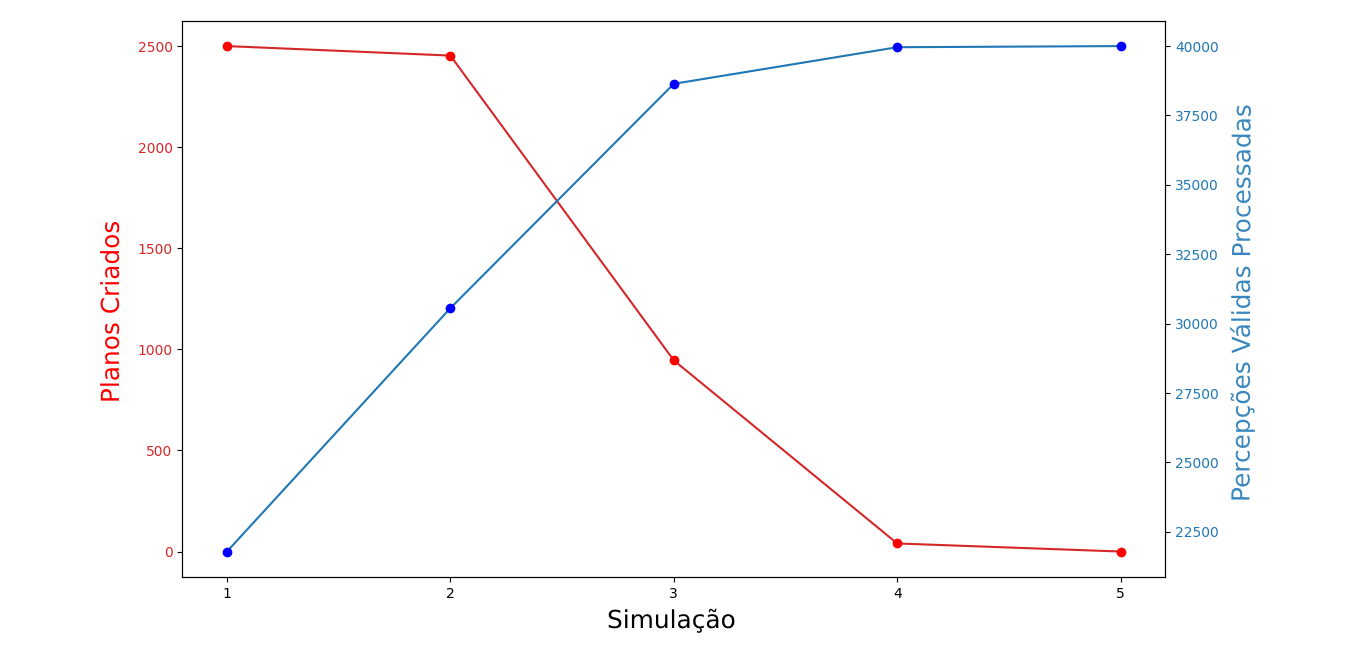
\includegraphics[width=\textwidth]{images/perceptions_vs_plans.png}
    \label{fig:perceptions_v_plans-experiment3}
    \caption{Evolução das percepções válidas processadas e dos planos novos criados ao longo das simulações.}
\end{figure}


\section{Conclusões e Trabalhos Futuros}

A ideia desse trabalho foi fazer uma revisão sistemática da literatura até então existente, apresentação de um modelo genérico para implementar a solução proposta e ter uma discussão dos benefícios, desafios e do futuro de segurança em internet das coisas, em específico do uso de técnicas da blockchain para tratar desses problemas. 

O modelo apresentado, que descreve os sistemas apresentados na revisão sistemática, pode servir como base para diversas implementações de sistemas de segurança para redes de internet das coisas utilizando blockchain. Apesar de servir muito bem, e já ter sido provado eficiente através de implementações iniciais, ainda existem problemas a serem resolvidos na área como um todo. A maior dificuldade, sem dúvida, é o alto consumo energético, derivado do requisito computacional que os algoritmos de segurança blockchain requerem, além da memória utilizada. Apesar do resultado da implementação específica ter sido muito satisfatório tanto em custo computacional quanto em custo energético, mais estudo na área é necessário para poder se chegar a conclusões concretas e que abranjam de maneira mais geral modelos segurança para redes do tipo. Como os sensores e microprocessadores utilizados pelas ``coisas'' nas redes de IoT serem muito simples, com baixo potencial computacional, baixa memória e necessidade de baixo consumo energético por questões térmicas, muito dos algoritmos de blockchain precisam ser revistos para que esse tipo de solução se torne simples de ser implantada e comum de ser vista nas redes domésticas, industriais e científicas.

O principal trabalho discutido em nossa revisão, e que foi utilizado como base para montarmos uma proposta concreta de solução genérica de segurança para internet das coisas utilizando blockchain \cite{dorri2017blockchain}, mostra como é possível fazer implementações do tipo, pois no trabalho realmente foi feita uma rede completa de internet das coisas para que os testes fossem realizados, tanto com blockchain quanto sem blockchain. Apesar do exemplo com blockchain ter apresentado resultados espetaculares com um custo de energia bem reduzido e tempo de resposta adicional quase desconsideráveis, mesmo que maior do que a implementação sem blockchain, que em questão de segurança era muito inferior devido a natureza simples das verficações de segurança e confiabilidade da rede, a replicação em larga escala do mesmo modelo ainda assim poderia trazer problemas por conta de um crescimento linear do custo. Mesmo assim, esse trabalho é pioneiro na área de otimização do tipo de solução apresentada, e tende a ser um tipo de trabalho a se repetir em novas esferas, com contextos diferentes e implementações ainda mais otimizadas que vão tornar possível a indústria aplicar esse tipo de solução a qualquer rede de coisas inteligentes a serem vendidas para o usuário final.

Em nosso trabalho apresentamos um modelo genérico, que possui certa validação mas que ainda pode ser aprimorado e testado arduamente para conseguir dados mais objetivos e relevantes para que a proposta como um todo se concretize como uma solução válida e implementável para redes de diversos tamanhos. Caso isso não aconteça, é certo que para determinados tipos e tamanhos de redes de internet das coisas o modelo funciona, então mesmo assim pode ser utilizado, apenas em empreitadas específicas e talvez reduzidas.

Portanto, os trabalhos futuros devem almejar não só a corretude da solução proposta, com modelos que já foram apresentados como funcionais por trabalhos anteriores, mas também focar na otimização das soluções para que tenham necessidade de menor custo computacional e consumo energético, para que em aplicações de larga escala a solução utilizando blockchain continue viável, mesmo com possivelmente milhões de coisas inteligentes interconectadas. Uma alternativa para essa solução é investir em soluções distribuídas, onde a computação pode ser distribuída de maneira eficiente através de algoritmos de distribuição de carga entre os diversos microprocessadores da rede IoT, extraindo o máximo potencial que essa tecnologia tem a oferecer com sua natureza de muitos dispositivos com pouco potencial de computação individual.

Além do avanço no trabalho atual como citado no parágrafo anterior, a arquitetura apresentada, bem como as contribuições que ela traz para a segurança em internet das coisas mesclando o crescente uso de controladores inteligentes com conceitos como blockchain, podem ser ainda mais mesclados com conceitos avançados de computação, IoT ou segurança. Um exemplo claro disso é a possibilidade de aplicar a técnica de Fog computing no modelo apresentado. Essa adição está fora do escopo do trabalho realizado, mas combina perfeitamente com a ideia de reduzir custo computacional de maneira geral na rede de internet das coisas e nesse caso específico para reduzir o custo computacional da implementação do Blockchain em um ambiente com diversos sensores transmitindo um grande volume de dados constantemente.

Por último, vale ressaltar a importância da transparência e da comunicação humana além das estratégias de segurança adotada. É crucial que o consumidor saiba que tipo de dados estão sendo coletados, e que tipo de sensores existem nos dispositivos inteligentes instalados em sua casa para que o relacionamento entre o consumidor e a rede utilizada seja saudável, despertando não só o interesse comercial com um aproveito unilateral por parte das empresas que provém esse tipo de serviço. Aviso da escolha, do mecanismo de acesso e da precisão da informação recolhida, políticas efetivas de minimização dos dados coletados e prestação de contas das medidas e falhas de segurança nos dispositivos são alguns fundamentos que tem se mostrado tendência por empresas que presam por um relacionamento saudável com o consumidor.


\bibliographystyle{sbc}
\bibliography{sbc-template}

\end{document}
